\documentclass[a4paper,12pt]{amsart}

\usepackage[T1]{fontenc}
\usepackage{graphicx}
\usepackage[polish]{babel}
\usepackage{tikz}
\usepackage{wrapfig}

\author[L. Moszczynski]{Lukasz Moszczynski}
\title[Obrazki]{Obrazki i rysunki}

\begin{document}
\maketitle
\begin{center}
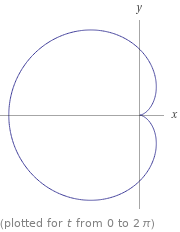
\includegraphics{obraz1.png}
\end{center}
\begin{center}
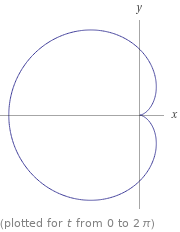
\includegraphics[scale=1.5]{obraz1.png}
\end{center}

Lorem ipsum dolor sit amet, consectetur adipiscing elit. Praesent ipsum libero, malesuada et consectetur auctor, fermentum ut mauris. Integer vitae est neque. Sed eu dignissim purus, et malesuada justo. Etiam non tortor est. Nunc vestibulum ex vitae massa feugiat condimentum. Praesent eu mattis lorem, at finibus nunc. Curabitur posuere nulla non cursus pharetra. Proin sed scelerisque ante. Nullam sagittis lobortis dui ut faucibus. Curabitur pretium arcu eros, et ullamcorper elit facilisis vel. Praesent elementum magna id quam ultricies, id ullamcorper lacus tempus. Vivamus ultrices hendrerit diam, a consequat libero bibendum ut. Nunc vitae metus in justo varius ultricies. In tincidunt scelerisque dapibus.

Duis at mattis tellus. Cras tempor blandit metus eget consectetur. Cras ut lacus elementum, sagittis massa id, rutrum enim. In interdum blandit orci. Interdum et malesuada fames ac ante ipsum primis in faucibus. Praesent posuere, risus sit ametvenenatis varius, arcu risus volutpat orci, at accumsan risus tellus sit amet turpis. Maecenas faucibus neque et dui condimentum malesuada cursus eget magna. Nunc viverra dui sodales rutrum gravida. Nullam eget lorem vitae est venenatis elementum nec sit amet ipsum.
\begin{center}
    
\includegraphics[width=360pt, height=70pt]{obraz2.png}
\end{center}
 Curabitur mollis sit amet risus eget eleifend. Vivamus tortor mi, fermentum id vehicula sit amet, sollicitudin sed nunc. Etiam interdum blandit est et mollis. Curabitur volutpat eleifend nunc eget gravida. Nunc placerat at odio id tristique.Nulla mattis enim a nulla posuere volutpat sit amet ac ipsum. In varius dapibus diam, sed blandit mauris laoreet sit amet.

Donec vitae tristique ante, in ultricies urna. Vestibulum scelerisque lorem nec mauris malesuada, eu ullamcorper sem fringilla. Fusce ultrices lacinia lectus eu tristique. In ut arcu vel ante gravida tristique a ut est. Vivamus id urna in augue blandit fringilla. Morbi iaculis placerat nibh vel interdum. Nullam vel erat ornare, tempus dui et, laoreet dolor.
\begin{figure}[h]
    \centering
    
\includegraphics[width=0.25\textwidth]{obraz2.png}
    \caption{OHANA MEANS FAMILLY}
    \label{fig:mesh1}
\end{figure}
Morbi eleifend neque at diam porttitor porttitor. asdf sadf Phasellus ante felis[ \ref{fig:mesh1} ],, varius sit amet pharetra posuere, scitu vut.[ \pageref{fig:mesh1} ]Donec consequat pellelolol AS ntesque tortor, nec auctor mauris volutpat vel. Aliquam in magna non libero elementum efficitur. Aenean tristique lobortis ante, vitae venenatis tellus vestibulum ac. Cras sit amet facilisis lectus. 
\begin{wrapfigure}{r}{0.5 \textwidth}
    
\includegraphics[width=5em]{obraz2.png}
    \caption{OHANA MEANS FAMILLY}
    \label{fig:mesh1}
\end{wrapfigure}
Aliquam sollicitudin in magna ac lacinia. Phasellus pharetra diam in orci facilisis condimentum. Aliquam mattis posuere mi, et scelerisque orci. Praesent ac posuere velit, at luctus dolor. Aliquam commodo consectetur quam id gravida. Cras quis venenatis risus. Integer id magna venenatis, sagittis nisi nec, semper ligula. Maecenas non ligula efficitur, posuere erat sed, pretium nisi. Donec at lacus orci. Vestibulum sit amet massa id massa finibus sodales.
\begin{figure}[h]
\begin{tikzpicture}[auto, node distance=2cm, thick, main node/.style={circle,draw,font=\small\bfseries}]
\node[main node](0){$u 0$};
\node[main node](1)[right of=0]{$u_1$};
\node[main node](2)[right of=1]{$u_2$};
\node[main node](3)[right of=2]{$u_k$};
\node[main node](4)[right of=3]{$u_n$};
\node[main node](5)[below of=4]{$v_n$};
\node[main node](6)[left of=5]{$v_k$};
\node[main node](7)[left of=6]{$v_2$};
\node[main node](8)[left of=7]{$v_1$};
\node[main node](9)[left of=8]{$v_0$};
\path[every node/.style={font=\small}]
(7) edge node [bend right]{$\gamma$}(8);
\path[every node/.style={font=\small}]
(8) edge node [bend right]{$\gamma$}(9);
\path[every node/.style={font=\small}]
(0) edge node [bend right]{$\alpha$}(1);
\path[every node/.style={font=\small}]
(1) edge node [bend right]{$\alpha$}(2);
\draw[-](3)to(6);
\draw[-](4)to(5);
\draw[-](2)to(7);
\draw[-](1)to(8);
\draw[-,dashed](2)to(3);
\draw[-,dashed](3)to(4);
\draw[-,dashed](5)to(6);
\draw[-,dashed](6)to(7);
\end{tikzpicture}
\end{figure}

\begin{figure}[h]
\centering
\begin{tikzpicture}[scale=0.5]
\path[draw=none,fill=blue,opacity=0.2](-8,-8)rectangle(8,8);
\draw[->](-8,0)--(8,0)node[below left]{$x$};
\draw[->](0,-8)--(0,8)node[below right]{$y$};
\draw[scale=1, domain=-2:2,smooth, variable=\y, blue]plot({\y^3},{\y});
\path[draw=none,fill=blue](4,-4)circle(2);
\path[draw=none,fill=blue](-4,4)circle(2);
\end{tikzpicture}
\caption{$y=\sqrt[3]x$ na $(-8,8)$}
\end{figure}

\end{document}